\begin{frame}{Gadżety}

\begin{columns}
\column{0.5\textwidth}
    Definiujemy relację w grafie przy~pomocy:
        \begin{itemize}
            \item relacji krawędzi \(E\)
            \item koniunkcji \(\land\)
            \item równości wierzchołków \(=\)
            \item kwantyfikatora \(\exists\)
        \end{itemize}

\column{0.5\textwidth}
    \begin{figure}
        \centering
        \begin{tikzpicture}[
    scale=0.5,
    line width=1pt,
    vertex/.style={
        circle,
        fill=black,
        inner sep=2.4pt
    },
    arr/.style={-{Triangle[length=2mm,width=1.5mm]}},
]

\node at (-7,-3) {\(P_3(u,v) \equiv\)};

\node[vertex, label=above:{\(u\)}]
    (p0) at (-4,1) {};
\node[vertex, label=right:{\(x\)}]
    (p1) at (-4,-1) {};
\node[vertex, label=right:{\(y\)}]
    (p2) at (-4,-3) {};
\node[vertex, label=below:{\(v\)}]
    (p3) at (-4,-5) {};

\draw[arr] (p0) -- (p1);
\draw[arr] (p1) -- (p2);
\draw[arr] (p2) -- (p3);

\end{tikzpicture}
    \end{figure}
    \vspace{-0.5em}
    \[ P_3(u,v) \equiv \exists_{x,y} \ E(u,x) \land E(x,y) \land E(y,v) \]
    \vspace{-2em}

\end{columns}

\end{frame}

% --------------------------------------------------------------

\begin{frame}{Gadżety w dowodzie}

    \vspace{-1em}
    \begin{figure}
        \centering
        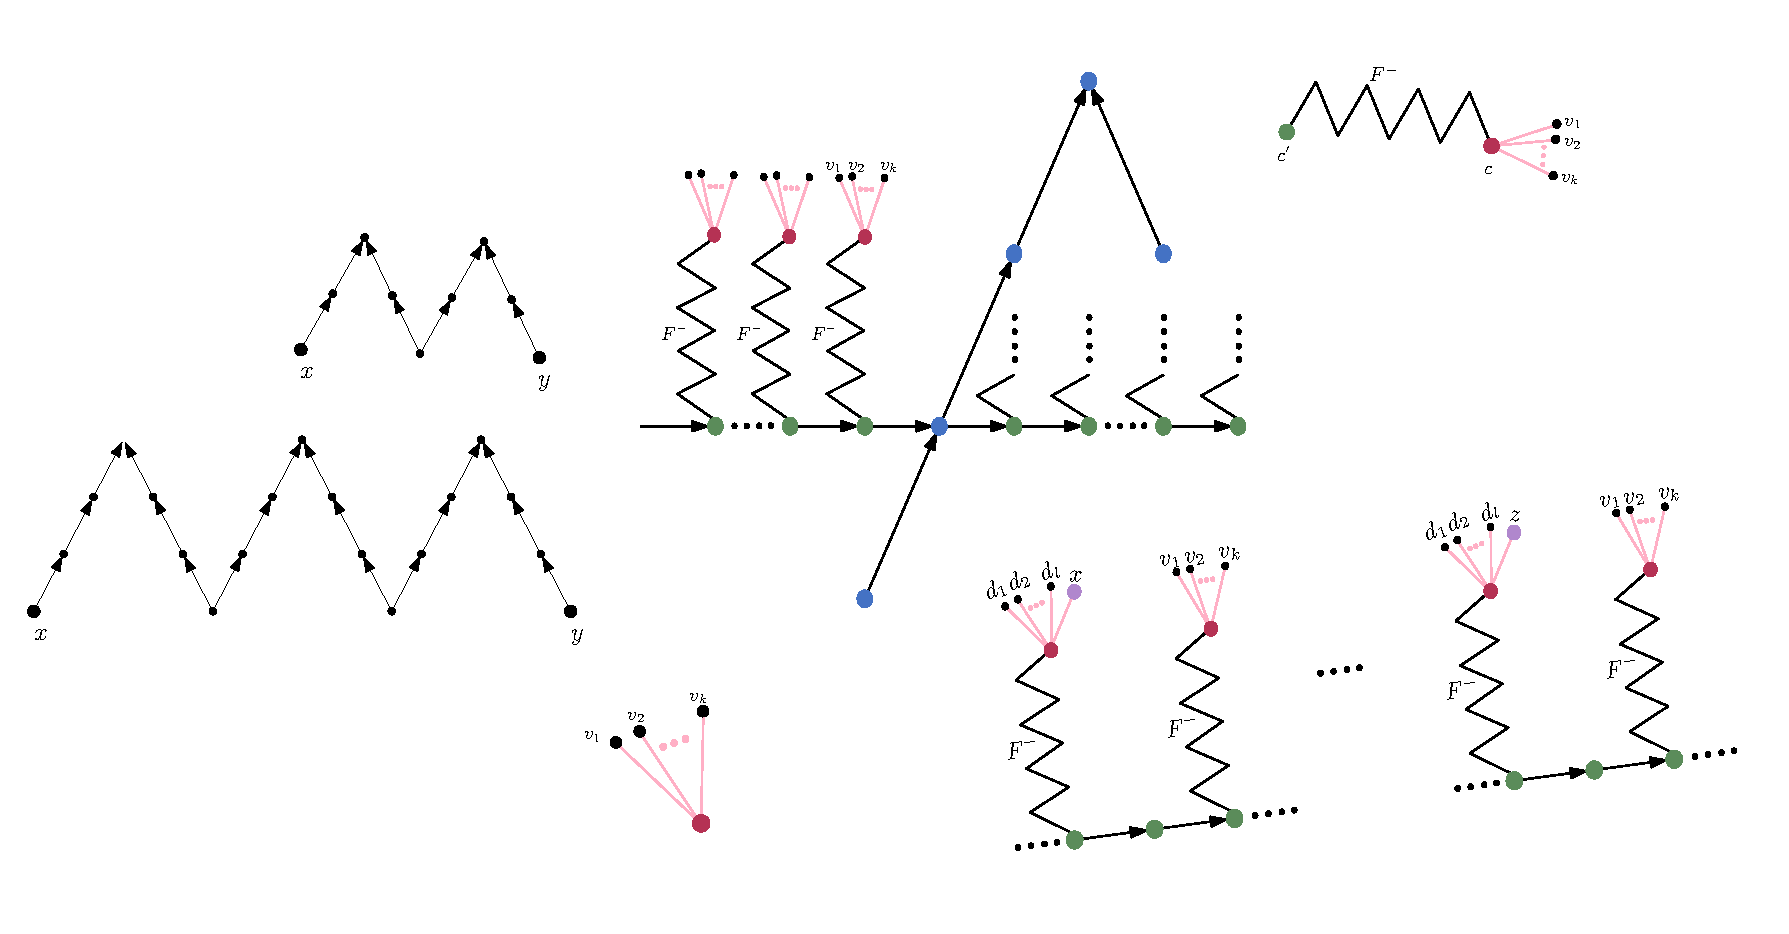
\includegraphics[width=1\linewidth]{img/gadget_gallery.pdf}
    \end{figure}

\end{frame}

% --------------------------------------------------------------

\begin{frame}{Rdzeń}

Rdzeń grafu \(G\) to najmniejszy jego podgraf, do którego \(G\) ma homomorfizm.

\vspace{1em}
\begin{figure}
    \centering
    \begin{tikzpicture}[
    scale=1.1,
    arr/.style={-{Triangle[length=2mm,width=1.5mm]}},
    minimum size=0.06cm,
    line width=1pt,
]

\begin{scope}[shift={(6,0)}]
    \node[circle, fill=cfteagreen!85]  (v1) at (0,2) {};
    \node[circle, fill=cfblue!85] (v2) at (2,2) {};
    \node[circle, fill=cfteagreen!85]  (v3) at (2,0) {};
    \node[circle, fill=cfblue!85] (v4) at (0,0) {};
    \node[circle, fill=cfred!85]  (v5) at (1,1) {};
    \draw[arr] (v2) -- (v1);
    \draw[arr] (v2) -- (v3);
    \draw[arr] (v4) -- (v3);
    \draw[arr] (v4) -- (v1);
    \draw[arr] (v5) -- (v2);
    \draw[arr] (v3) -- (v5);
    \node at (1,-1) {\(G\)};
    \node at (3.6,1) {\(\core(G)\)};
\end{scope}

% highlight
\begin{scope}[on background layer]
    \fill[cfgrey!40, rounded corners=20pt]
        ([shift={(-1,0)}] v5.center) --
        ([shift={(0.5,1)}] v2.center) --
        ([shift={(0.5,-1)}] v3.center) --
        cycle;
\end{scope}

\end{tikzpicture}
\end{figure}

\end{frame}


% --------------------------------------------------------------

\begin{frame}{Gadżety -- szablon rdzenia}

    Jeśli \((v_1, \dots, v_k) \in \core\), to \(v_1, \dots, v_k\) indukują podgraf izomorficzny z rdzeniem grafu \(G\) \linebreak dla ustalonej numeracji wierzchołków rdzenia \(q_1,\dots,q_k\).

\vspace{1.5em}
\begin{columns}
\column{0.65\textwidth}
    \[ \core(v_1,\dots,v_k) \equiv \bigwedge_{q_i q_j \in E} E(v_i,v_j) \]

\column{0.65\textwidth}
    \begin{tikzpicture}[
    scale=0.9,
    line width=1pt,
    arr/.style={-{Triangle[length=2mm,width=1.5mm]}},
    arr2/.style={{Triangle[length=2mm,width=1.5mm]}-{Triangle[length=2mm,width=1.5mm]}},
    minimum size=0.06cm
]

\node[circle, fill=cfblue!85, inner sep=2.8pt, label=left:{\(q_1\)}]
    (v1) at (0,0.2) {};
\node[circle, fill=cfblue!85, inner sep=2.8pt, label=right:{\(q_2\)}]
    (v3) at (2,0.2) {};
\node[circle, fill=cfblue!85, inner sep=2.8pt, label=above:{\(q_3\)}]
    (v2) at (1,1.8) {};

\draw[arr] (v1) -- (v2);
\draw[arr] (v2) -- (v3);
\draw[arr2] (v1) -- (v3);

\end{tikzpicture}
\end{columns}

\end{frame}



% --------------------------------------------------------------

\begin{frame}{Przykład -- szablon rdzenia}

\begin{columns}
\column{0.5\textwidth}
    \begin{figure}
        \centering
        \begin{tikzpicture}[
    scale=1,
    line width=1pt,
    arr/.style={-{Triangle[length=2mm,width=1.5mm]}},
    arr2/.style={{Triangle[length=2mm,width=1.5mm]}-{Triangle[length=2mm,width=1.5mm]}},
    minimum size=0.06cm
]

\begin{scope}[shift={(11,0)}]
    \node[circle, fill=cfblue!85, label=left:{\(u\)}]
        (v1) at (0,0.2) {};
    \node[circle, fill=cfblue!85, label=right:{\(v\)}]
        (v3) at (2,0.2) {};
    \node[circle, fill=cfblue!85, label=above:{\(w\)}]
        (v2) at (1,1.8) {};

    \draw[arr] (v1) -- (v2);
    \draw[arr] (v2) -- (v3);
    \draw[arr2] (v1) -- (v3);

    \node at (1,-1) {rdzeń bez automorfizmów};
\end{scope}

\end{tikzpicture}
    \end{figure}

\column{0.5\textwidth}
    \begin{align*}
        \core(u,v,w)&\equiv E(u,v) \land E(v,u) \\
        &\land E(u,w) \\ 
        &\land E(w,v)
    \end{align*}
    \[ \core = \set{(u,v,w)} \]
\end{columns}

\vspace{1em}
\onslide<2->{
    \[ R_u(x) \equiv \exists_{v_1, v_2, v_3} \ \core(v_1, v_2, v_3) \land E(x, v_1) \]
}

\end{frame}

% --------------------------------------------------------------

\begin{frame}{Przykład -- szablon rdzenia}

\begin{columns}
\column{0.5\textwidth}
        \begin{figure}
            \centering
            \begin{tikzpicture}[
    scale=1,
    line width=1pt,
    arr/.style={-{Triangle[length=2mm,width=1.5mm]}},
    minimum size=0.06cm,
]

\begin{scope}[shift={(11,0)}]
    \node[circle, fill=cfred!85, label=left:{\(u\)}]
        (v1) at (0,0.2) {};
    \node[circle, fill=cfred!85, label=right:{\(v\)}]
        (v3) at (2,0.2) {};
    \node[circle, fill=cfred!85, label=above:{\(w\)}]
        (v2) at (1,1.8) {};

    \draw[arr] (v1) -- (v2);
    \draw[arr] (v2) -- (v3);
    \draw[arr] (v3) -- (v1);

    \node at (1,-1) {rdzeń z automorfizmami};
\end{scope}

\end{tikzpicture}
        \end{figure}

\column{0.5\textwidth}
    \begin{align*}
        \core(u,v,w)&\equiv  E(v,u) \\
        & \land E(u,w) \\ 
        & \land E(w,v)
    \end{align*}
    \begin{tikzpicture}
    \node (a) {\(\core = \set{(u,v,w), (v,w,u),(w,v,u)}\)};
    \node[below=0.5cm of a] (b) {\textcolor{cfred}{Przez automorfizmy nie mamy stałych.}};
    \draw[->, thick, cfred] (a.west) to[bend right] (b.north west);
    \end{tikzpicture}
\end{columns}

\vspace{1em}
\onslide<2->{
    \[ R_u(x) \equiv \exists_{v_1, v_2, v_3} \ \core(v_1, v_2, v_3) \land E(x, v_1) \]
}

\end{frame}

% -----------------------------------------------------------

\begin{frame}{Przykład -- wiele kopii}

\begin{columns}
\column{0.5\textwidth}
        \begin{figure}
        \centering
        \begin{tikzpicture}[
    scale=0.9,
    line width=1pt,
    arr/.style={-{Triangle[length=2mm,width=1.5mm]}},
    arr2/.style={{Triangle[length=2mm,width=1.5mm]}-{Triangle[length=2mm,width=1.5mm]}},
    minimum size=0.06cm
]


\begin{scope}[shift={(11,0)}]

    \node[circle, fill=cfred!85, label=above:{\(u\)}]
        (v1) at (0,-0.2) {};
    \node[circle, fill=cfblue!85, label=below:{\(w\)}]
        (v2) at (1,-1.8) {};
    \node[circle, fill=cfblue!85, label=above:{\(v\)}]
        (v3) at (2,-0.2) {};

    \draw[arr] (v1) -- (v2);
    \draw[arr] (v2) -- (v3);
    \draw[arr2] (v1) -- (v3);

    \node[circle, fill=cfred!85, label=left:{\(u'\)}]
        (v4) at (3,-1.5) {};
    \node[circle, fill=cfblue!85, label=above:{\(w'\)}]
        (v5) at (4,0.1) {};
    \node[circle, fill=cfblue!85, label=right:{\(v'\)}]
        (v6) at (5,-1.5) {};

    \draw[arr] (v4) -- (v5);
    \draw[arr] (v5) -- (v6);
    \draw[arr2] (v4) -- (v6);

    \node[circle, fill=cfblue!85, label=below:{\(w''\)}]
        (v7) at (4,-3.1) {};

    \draw[arr] (v6) -- (v7);
    \draw[arr] (v7) -- (v4);
    \draw[arr] (v2) -- (v7);
    \draw[arr] (v5) -- (v3);

    \begin{scope}[on background layer]
        \fill[cfgrey, opacity=0.25, draw=cfgrey, rounded corners=20pt]
            ([shift={(-1,-0.5)}] v4.center) --
            ([shift={(0,1)}] v5.center) --
            ([shift={(1,-0.5)}] v6.center) --
            cycle;

        \fill[cfgrey, opacity=0.25, draw=cfgrey, rounded corners=20pt]
            ([shift={(-1,0.5)}] v4.center) --
            ([shift={(0,-1)}] v7.center) --
            ([shift={(1,0.5)}] v6.center) --
            cycle;

        \fill[cfgrey, opacity=0.25, draw=cfgrey, rounded corners=20pt]
            ([shift={(-1,0.5)}] v1.center) --
            ([shift={(0,-1)}] v2.center) --
            ([shift={(1,0.5)}] v3.center) --
            cycle;
    \end{scope}

\end{scope}

\end{tikzpicture}
    \end{figure}
        
\column{0.5\textwidth}
    \begin{align*}
        \core(u,v,w)&\equiv  E(v,u) \\
        & \land E(u,w) \\ 
        & \land E(w,v)
    \end{align*}
    \begin{tikzpicture}
    
    \node (a) {\(\core = \set{(u,v,w), (u',v',w'),(u',v',w'')}\)};
    \node[below=0.5cm of a] (b) {\textcolor{cfred}{Mamy stałe w obrębie kopii rdzenia.}};
    \draw[->, thick, cfred] ([xshift=3pt]a.south west) to[bend right] (b.west);
    \end{tikzpicture}
\end{columns}

\vspace{1em}
\onslide<2->{
    \[ R_u(x) \equiv \exists_{v_1, v_2, v_3} \ \core(v_1, v_2, v_3) \land E(x, v_1) \]
}

\end{frame}

% -----------------------------------------------------------

\begin{frame}{Problem -- wiele kopii}

    \[ \alpha(x, y) \iff \underset{\text{kopia rdzenia}}{\exists_{v_1, \dots, v_k} \ \core(v_1, \dots, v_k)} \land R(x, y, v_1) \dots \land R(x, y, v_k) \]

\begin{columns}
\column{0.35\textwidth}
    \begin{figure}
        \centering
        \begin{tikzpicture}[
    scale=0.85,
    line width=1pt,
    arr/.style={-{Triangle[length=2mm,width=1.5mm]}},
    arr2/.style={{Triangle[length=2mm,width=1.5mm]}-{Triangle[length=2mm,width=1.5mm]}},
    minimum size=0.06cm,
    inner sep 2.6pt,
]

\node[circle, fill=cfred!85, label=left:{\(u\)}]
    (v1) at (0,0) {};
\node[
    circle,
    minimum size=8pt,
    path picture={
        \fill[cfblue!85]
            (path picture bounding box.south west)
            rectangle
            (path picture bounding box.north);
        \fill[cfred!85]
            (path picture bounding box.south)
            rectangle
            (path picture bounding box.north east);
    },
    label=left:{\(v\)}
] (v2) at (0,2) {};
\node[circle, fill=black, inner sep=2.4pt]
    (v3) at (2,2) {};
\node[circle, fill=black, inner sep=2.4pt]
    (v4) at (2,0) {};

\draw[arr] (v1) -- (v2);
\draw[arr] (v2) -- (v3);
\draw[arr] (v3) -- (v4);
\draw[arr] (v4) -- (v1);
\draw[arr] (v1) -- (v3);

% \begin{scope}[on background layer]
%     \fill[cfgrey, opacity=0.25, draw=cfgrey, rounded corners=20pt]
%         ([shift={(-0.5,-0.5)}] v1.center) --
%         ([shift={(-0.5,0.5)}] v2.center) --
%         ([shift={(0.5,0.5)}] v3.center) --
%         ([shift={(0.5,-0.5)}] v4.center) --
%         cycle;
% \end{scope}

\node[circle, fill=cfblue!85, label=left:{\(w\)}]
    (u3) at (-1,3.6) {};
\node[circle, fill=black, inner sep=2.4pt]
    (u4) at (0.9,4.6) {};
\node[circle, fill=black, inner sep=2.4pt]
    (u5) at (1.85,2.9) {};

\draw[arr] (v2) -- (u3);
\draw[arr] (u3) -- (u4);
\draw[arr] (u4) -- (u5);
\draw[arr] (u5) -- (v2);
\draw[arr] (v2) -- (u4);

\end{tikzpicture}
    \end{figure}

\vspace{1em}
\column{0.65\textwidth}
    \!Przechodniość: \\[-1.25em]
    \[ \alpha(u,v) \text{ i } \alpha(v, w) \overset{\text{?}}{\implies} \alpha(u, w) \]

    \onslide<2>{
    Domykamy przechodnio relację \(\alpha\): \\[-2.25em]
    \begin{align*}
        \alpha'(x,y) \equiv \exists_{z_1, \dots, z_i} \ \alpha(x, z_1)
        \land \alpha(z_1, z_2) \land \dots \land \alpha(z_i, y)
    \end{align*}
    }
\end{columns}

\end{frame}

% -----------------------------------------------------------

\begin{frame}{Gadżety -- definiowalny podgraf}

\begin{columns}
\column{0.45\textwidth}
    \begin{tikzpicture}[
    scale=1.1,
    arr/.style={-{Triangle[length=2mm,width=1.5mm]}},
    arr2/.style={{Triangle[length=2mm,width=1.5mm]}-{Triangle[length=2mm,width=1.5mm]}},
    line width=1pt,
    inner sep=2.8pt,
]

\node[circle, fill=black] (v1) at (0,2) {};
\node[circle, fill=cfblue!85] (v2) at (2,2) {};
\node[circle, fill=cfblue!85, label=below:{\(u\)}] (v3) at (2,0) {};
\node[circle, fill=black] (v4) at (0,0) {};
\node[circle, fill=cfblue!85] (v5) at (1,1) {};
\draw[arr] (v2) -- (v1);
\draw[arr2] (v3) -- (v2);
\draw[arr] (v4) -- (v3);
\draw[arr] (v4) -- (v1);
\draw[arr] (v2) -- (v5);
\draw[arr] (v5) -- (v3);
\node at (3.6,1) {\(G'=(V', E')\)};

% highlight
\begin{scope}[on background layer]
    \fill[cfgrey!40, rounded corners=20pt]
        ([shift={(0.5,0.8)}] v2.center) --
        ([shift={(0.5,-0.5)}] v3.center) --
        ([shift={(-0.8,-0.5)}] v4.center) --
        cycle;
\end{scope}

\end{tikzpicture}

\column{0.45\textwidth}
    Definiujemy gadżetowo \(G'\) podgraf \(G=(V,E):\)
    \begin{align*}
        &V'(x) \equiv \exists_{v_1, v_2, v_3} \ \core(v_1, v_2, v_3) \land E(x, v_1) \\
        &E'(x,y) \equiv V'(x) \land V'(y) \land E(x,y)
    \end{align*}
\end{columns}

\end{frame}
